% \begin{savequote}[75mm]
% Nulla facilisi. In vel sem. Morbi id urna in diam dignissim feugiat. Proin molestie tortor eu velit. Aliquam erat volutpat. Nullam ultrices, diam tempus vulputate egestas, eros pede varius leo.
% \qauthor{Quoteauthor Lastname}
% \end{savequote}

\chapter{Object representations in lateral visual cortex}
\newthought{Shape is a diagnostic feature} of object identity. Visually similar objects, such as a pear and an apple, can be grouped together by certain shared visual features. On the other hand, different images or views of any one object can look dramatically dissimilar, yet still belong to the same object. The ventral visual pathway in the primate brain is thought to transform non-diagnostic, low-level representations of features that may be common to many different objects into high-level representations that are both diagnostic of object identity, or selective for a given object, and robust to variations in particular appearance, or tolerant to identity-preserving transformations. In the first chapter, we established the behavioral ability of rats to perform visual object recognition and quantified their perceptual choices of object similarity. We next turned our attention to the neuronal substrates of these abilities. 

% Neural subtrates of object recog. -- what do we know from primates.
Primate visual cortex is arranged hierarchically, with visual inputs from the thalamus first arriving in so-called ``striate'' cortex (also known as area V1), before being processed and forwarded through a successive chain of hierarchically-organized visual areas (area V2 < area V4 < IT) along the ventral surface of the brain. Along each stage of the ventral stream, there is a gradual increase in object selectivity and tolerance, culminating in area IT, at the highest level of the ventral pathway. 

Several key trends have been observed in the response properties of visual neurons as one progresses from ``lower'' to ``higher'' visual areas along this ventral pathway. First, the region of visual space that a given cell responds to (the ``receptive field'') gradually increases as one moves along the ventral pathway, with receptive fields in the highest stages of visual cortex sometimes responding to up to half of the visual field\cite{OpDeBeeck2001}. Meanwhile, selectivity for complex object features also increases along the ventral visual pathway, with neurons in later stages of the pathway responding only to very particular configurations of features\cite{Desimone1984, Logothetis1996}. Critically, as one progresses along the ventral pathway, neurons also exhibit greater tolerance to identity-preserving transformation of the retinal image -- that is, neurons tend to retain their selectivity for particular object features even if those features are, for instance, moved around on the retina, or scaled up or down in size\cite{Ito1995}.These combined features of selectivity and tolerance are in many ways the key computational hallmarks of high-level vision\cite{DiCarlo2007, DiCarlo2012}. 

% Previous rodent studies
% \section{Lateral visual cortex exhibits some of the same core properties found in primates}
Anatomical studies have shown that the connectivity of rodent visual cortex observes a similar hierarchical pattern, with thalamic inputs arriving in an analogous striate area V1 in posterior of the brain, and then projecting ventrally to a series of interconnected extrastriate areas\cite{Coogan1993}. However, while these areas have been characterized anatomically, much less is known about their function. Most of what we know about rat visual cortex beyond V1 comes from single-unit, electrophysiology studies that have characterized response properties of neurons in the context of visual object recognition\cite{Tafazoli2017, Vermaercke2014, Vinken2014}. A few key trends have been observed. First, all studies to date report an increases in receptive field size from V1 to LM to LI and beyond\cite{Tafazoli2017}. This is consistent with studies of extrastriate cortex in mice\cite{Murgas2020, Siegle2021}, as well as my characterizations from the previous chapter. Second, though there is not yet a clear consensus, several studies report increased shape selectivity or shape discriminability for single-units in extrastriate cortex\cite{Tafazoli2017, Vermaercke2014, Vermaercke2015, Vinken2016}. Finally, most studies report some degree of tolerance to identity-preserving transformations: single-units recorded in extrastriate cortex along these lateral areas maintain shape selectivity or discriminability across changes in position, size, or rotation\cite{Vermaercke2014, Tafazoli2017}.

At the same time, mouse visual cortex has been characterized to an unprecedented degree, such that arguably more is known about the mouse visual system that that of any primate (see \citet{Niell2021} for a review). Despite many apparent similarities between rodent and primate visual system, these studies present a growing body of discoveries on the many ways in which the two are significantly different. For example, several studies have found asymmetries in visual field representations and direction tuning preferences in mouse visual cortex\cite{Zhuang2017, Liang2018, Sit2020, Murgas2020}. In addition, the deep, hierarchical organization evident in primate visual cortex seems to be quite different in rodent visual cortex. For example, postrhinal cortex ( POR), a higher-order visual area in the mouse, receives most visual input via the superior colliculus (SC), and not V1 by way of the dLGN --- silencing V1 activity does not affect motion-processing activity of POR cells\cite{Beltramo2019}. This means that unlike the traditional view of information flow in the visual system, where V1 is the gateway through the ventral path, mice have a separate pathway to higher-order visual areas. Thus, in the context of visually-driven behavior, rodent and primate visual systems may have different principles of organizations or species-specific solutions for a given behavioral need. 

To determine the extent to which rat lateral visual cortex intrinsically exhibits properties thought to be important for spontaneous, as opposed to learned, object recognition behavior, I recorded from neural populations in awake, naive rats presented with a subset of the same stimuli tested on the trained rats (see Chapter 1, Figure\ref{fig:behavior_generalization}). The goal of these experiments was to investigate how neural responses reflect changes in shape that are due to transformations along identity-changing axes or transformations along identity-preserving axes.

% ---------------------------------------------------------------
% Single neuron selectivity and tolerance
% ---------------------------------------------------------------
\section{Selectivity and tolerance of single neurons}
\begin{figure}[hbt!]
    \includegraphics[width=0.9\textwidth]{figures/chapter_4/fig_4-1_single_cell_selectivity_tolerance/fig_4-1_single_cell_selectivity_tolerance.pdf}
    \caption[Single neuron selectivity and tolerance]{Selectivity and tolerance metrics for single neurons. 
    \textbf{A.} Transformations tested: 5 stimulus sizes (identity-preserving) and 9 morph levels (identity-changing). 5 full-field (FF) stimuli with a constant gray-scale value were matched in overall luminance to each size (see Methods).
    \textbf{B.} Rat visual areas in this study. 
    \textbf{C.} Morph selectivity (left) and size tolerance (right) for an example V1 FOV. Black lines, single cell tuning profiles. Colored lines, example cells. Green, the first set of traces (middle). Purple, the lower set (bottom). Time courses arranged as in \textbf{A}, luminance not shown. Solid black lines and shading, mean and SEM across repetitions.
    \textbf{D.} Same as \textbf{C}, but for an LM FOV.
    \textbf{E.} Same as \textbf{B} and \textbf{C}, but for an LI FOV.
    \textbf{F.} Distributions of size tolerance for V1, LM, and LI cells. Each dot is a cell. Black horizontal and vertical bars, mean and SD across cells.
    \textbf{G.} Same as \textbf{F}, but for morph selectivity. 
    \textbf{H.} Correlation between size tolerance and morph selectivity for example V1, LM, and LI FOVs. Each dot is a cell. Solid black line and shading, linear fit and 95\% CI.
    \label{fig:selectivity_tolerance}}
\end{figure}

One key feature of the primate ventral stream is a gradual increase in shape or object selectivity and a parallel increase in tolerance to identity-preserving transformations. Previous studies have shown that single-units in area IT of monkeys exhibit a trade-off between these properties: neurons that are highly selective are less tolerant to identity-preserving transformations and highly tolerant neurons are not as selective to particular objects\cite{Zoccolan2007}.

To determine whether single neurons exhibited similar characteristics in rat visual areas, I first measured single neuron response profiles in areas V1, LM, and LI. For identity-changing transformations, I tested a subset of the morphs used to test the naive perceptual boundaries between the anchor objects in trained animals (Figure\ref{fig:selectivity_tolerance}A). For identity-preserving transformations, I tested a subset of sizes covering the range of stimulus sizes used to test behavioral generalization performance (see Chapter 1, Figure\ref{fig:behavior_generalization}). Since size changes come with large changes in luminance, I also presented a subset of full-screen stimuli that were assigned luminance-matched gray-scale values for each size tested (see Methods).

All areas contained a diverse range of object selective and size tolerant cells. For example, some cells exhibited size tuning but did not respond differently to the various morphs, while other cells exhibited tuning to particular morphs, without showing response modulation to the different sizes. Still others appeared to be tuned to overall luminance, showing selective responses to the full-screen stimuli and no responses to shapes. Overall, I found that across the tested object stimuli, cells in LI had the lowest lifetime sparseness, while cells in V1 and LM were similarly high in sparseness (Mann-Whitney U-test, p<0.01, corrected for multiple comparisons with the Benjamini/Hochberg method). Since changes in object shape were due to both variation in morph level and in stimulus size, the sparseness observed in V1 and LM could reflect a higher selectivity for morph shapes or a lower tolerance to varying size. To quantify the amount of object selectivity and tolerance, I calculated a morph selectivity index (MX) and a size tolerance index (ST) for each cell\cite{Zoccolan2007}. I found a range of tuning profiles across cells that was comparable between the three areas (Figure\ref{fig:selectivity_tolerance}B-D). On average, LI cells were both less selective to morph shape and more tolerant to changes in size, relative to cells in V1 and LM (Figure\ref{fig:selectivity_tolerance}E-F). Notably, this difference was not attributable to overall lower response magnitudes in LI: although there were relatively fewer LI cells responsive to the object stimuli overall, of the cells that were responsive, response magnitudes were comparable across areas (see Table\ref{tab:data_counts}).

It is possible that the relatively higher average morph selectivity in V1 and LM cells reflects greater sensitivity to overall luminance values. To characterize the extent to which size or morph tuning simply tracks luminance sensitivity, I compared tuning for size to tuning for the full-screen luminance stimuli. Specifically, I calculated the correlation between each cell's tuning curve for all sizes for its preferred morph object, and its tuning curve for the size-matched luminance stimuli. While there were indeed cells whose size- or morph-tuning profiles were tightly correlated with broad luminance levels, this was not the case for the majority of cells (V1: 9.8+/-6.8\% of cells with significant correlation between size and luminance tuning; LM: 12.6+/-8.2\%; Li: 12.2+/-9.1\%, see Figure\ref{supfig:luminance_corr}). 

To determine whether single neurons in rat visual cortex exhibit a similar trade-off between shape selectivity and transformation tolerance as observed in primate IT, I calculated the correlation between morph selectivity and size tolerance for simultaneously recorded cells in each imaging site (Figure\ref{fig:selectivity_tolerance}H). I found a strong, negative correlation between morph selectivity and size tolerance for areas LM and LI. Notably, these features were also negatively correlated in V1 imaging sites, but to a weaker degree. To determine whether the strength of this trade-off differed between the three areas, I performed a shuffle test in which I scrambled each cell’s selectivity index and tolerance index, then recalculated the trade-off metric (correlation coefficients). When comparing populations that passed this shuffle test (p<0.05 over 5000 iterations), I found that correlation coefficients for LM and LI populations were significantly more negative than those in area V1 (Mann-Whitney U test, p<0.05 Bonferroni-corrected for multiple comparisons), suggesting that on average, the negative relationship between selectivity and tolerance was stronger for LM and LI FOVs.

% A critical property of single neurons in IT is the preservation of rank-ordered object selectivity, that is, relative tuning preference for a set of objects is maintained across changes in identity-preserving transformations such as position or size\cite{Li2009, REFREF}. 

% ---------------------------------------------------------------
% Arousal
% ---------------------------------------------------------------
\section{Arousal modulation of tuning properties} 
\begin{figure}[t!]
    \includegraphics[width=\textwidth]{figures/chapter_4/fig_4-2_arousal/fig_4-2_arousal.pdf}
    %\vspace{.1in}
    \caption[Arousal modulates tuning]{Arousal modulates tuning. 
    \textbf{A.} Example view of the face-tracking camera pointed at the animal’s face, overlaid with face feature annotations for whiskers and pupil tracking.
    \textbf{B.} Example pupil diameter trace (top) and neural responses (bottom) for repeated presentations of a single condition type. Gray bars in the middle show the stimulus period of each trial. Color map shows z-scored responses.
    \textbf{C.} Response magnitude on trials in which animals were in “high” (magenta) and “low” (cyan) arousal states (i.e. trials with an average pupil diameter above or below the 67th and 33rd percentiles, respectively). Points, average response magnitude across cells of a given imaging site. Error bars, SD.
    \textbf{D.} Size tolerance as a function of arousal state, for each visual area. Points, average response magnitude across cells of a given imaging site. Horizontal bars, average across sites for a given visual area. Error bars, SD.
    \textbf{E.} Morph selectivity as a function of arousal state, for each visual area. Notation as in \textbf{E}.
    \textbf{F.} Correlation coefficient for morph selectivity versus size tolerance as a function of arousal state, for each visual area. Notation as in \textbf{E}, \textbf{F}.
    \label{fig:arousal}}
\end{figure}

Tuning preferences are known to be modulated by the behavioral state of the animal, such as overall arousal or locomotion\cite{Niell2010,Saleem2013,Vinck2015, Dadarlat2017}. Even in the absence of visual stimulation, neural activity in visual cortex can be driven and modulated by locomotion or facial movements\cite{Keller2012SensorimotorMouse, Stringer2019spontaneous}. A key advantage of recording in head-fixed rats was the ability to simultaneously monitor facial movements of the animals with (Figure\ref{fig:arousal}A-B). Face video was acquired simultaneously and synced with neural acquisition (see Methods). From these data, a rich repertoire of facial and front-of-body movements could be extracted for every frame, including eye position, pupil size, whisker positions, snout and mouth locations, as well as paw positions. These features were extracted\cite{Mathis2018, Nath2019} and aligned to neural activity, as I designed the acquisition pipeline to sync with that of the neural acquisition pipeline (see Supplementary Information).

% pupil 
Decades of research in pupillometry in humans, nonhuman primates, and rodents support the view that changes in pupil diameter track not only changes in luminance, but also changes in alertness, attention, and effort, or broadly, levels of arousal\cite{Reimer2016, McGinley2015WakingResponses, Reimer2014, Vinck2015}. Arousal states, as measured by methods from pupillometry, have been shown to modulate both single neuron tuning and population decoding. To characterize how broad changes in arousal modulate the visual response properties of cells tuned to the object stimuli, I compared neural activity between high and low arousal states, as measured by changes in pupil size\cite{Liang2020, Stringer2019spontaneous}. Specifically, trials were separated into ``high'' or ``low'' states based on pupil size. Since pupil diameter changes with luminance changes, as well, care was taken to sample the range of pupil sizes within each stimulus condition (see Methods). 

I compared single cell measures of size tolerance and shape selectivity, as well as linear separability of population representations across areas V1, LM and LI. Consistent with previous studies of arousal modulation in V1, I found that response magnitudes were greater when the animal was in a high arousal state, as compared to a low arousal state, and this was also true for areas LM and LI (Figure\ref{fig:arousal}C). Across these visual areas, shape selectivity was also greater, and size tolerance lower, in high arousal states (Figure\ref{fig:arousal}D-E). That is, increased arousal was correlated with overall increases in selectivity.

To see whether the previously observed trade-off between selectivity and tolerance was modulated by arousal, I also quantified the correlation between the two for high and low arousal states. Interestingly, in V1, but not in LM and LI, the strength of this relationship, as measured by the size of the correlation coefficient between tolerance and selectivity, was weaker in high arousal states (Figure\ref{fig:arousal}F). The reduced strength of the negative correlation between selectivity and tolerance may be predictable if, on average, increases in morph selectivity result in increases in size tolerance (\textit{i.e.}, a less steep slope for the correlation plots shown in Figure\ref{fig:selectivity_tolerance}H). However, that this is not evident in LM and LI populations, despite all three areas exhibiting similar increases in selectivity for high arousal states, suggest that these populations are relatively more robust to arousal differences at the level of individual cells. 

% ---------------------------------------------------------------
% Morphs
% ---------------------------------------------------------------
\section{Object discrimination in single neurons}
% Morphs -- neurometric curves, single-neuron disriminability
% 
Overall, though I observed a slight increase in size toleranace and a slight decrease in morph selectivity comparing across areas V1 to LM to LI, the distributions of selectivity and tolerance metrics were broad and otherwise quite similar for all there areas. One concern with the observation that the greater size tolerance in LI could be due to LI cells simply not having any preference at all for the particular shapes being presented, despite being visually responsive.  
I previously showed that trained rats are capable of discriminating between object A and object B, and that their determination of the morph shapes varied as a function of how similar a given morph shape was to either A or B (see Figure\ref{fig:behavior_generalization}). However, in the naive rats, there was no reason for cells to prefer one object over the other. Nonetheless, it was possible to quantify the extent to which a given cell intrinsically, or at least, without training or experience, demonstrates strong selectivity for one or the other shapes, based on its ability to discriminate between the stimuli.

\begin{figure}[hbt!]
    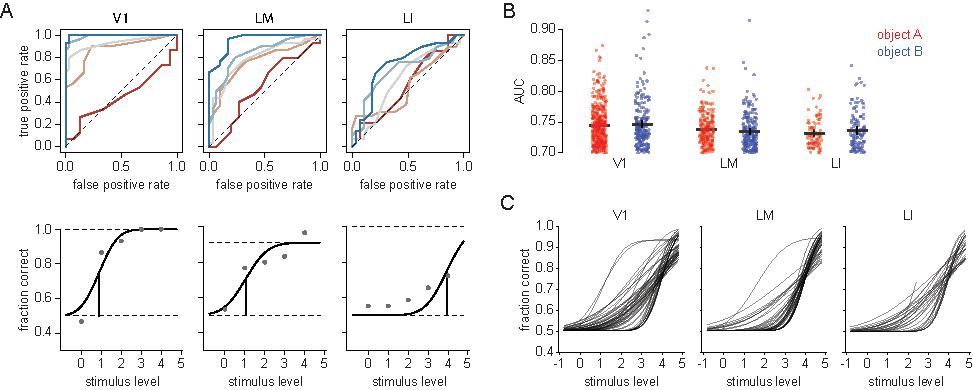
\includegraphics[width=\textwidth]{figures/chapter_4/fig_4-3_neurometric/fig_4-3_neurometric.pdf}
    %\vspace{.1in}
    \caption[Single neuron discriminability]{Single neuron discriminability. 
    \textbf{A.} Distribution of discriminability (AUC) for cells selective for either object A (red) or object B (blue), which were the two anchor objects.
    \textbf{B.} \textit{Top}, Example time courses at each morph level at the preferred size for a cell preferring object B. \textit{Bottom}, Example time courses for a cell preferring object A. Horizontal bar, stimulus period. 
    \textbf{C.} \textit{Top}: Example ROC curves for the cell shown in \textbf{B}, \textit{top}. The area under these curves (AUC) measures how well a neuron discriminates one image, the preferred object B, from each other image, or the other morph levels. Red corresponds to object A (morph level 0\%B) and blue corresponds to object B (morph level 100\%B). \textit{Bottom}: ROC curves, but for the cell shown in \textbf{B}, \textit{bottom}. 
    \textbf{D.} \textit{Top}: Corresponding neurometric curves fit to the AUC values (``accuracy'') at each morph level for the cell shown in the top panels of \textbf{B} and \textbf{C}. \textit{Bottom}: Corresponding neurometric cures for the cell shown in the bottom panels of \textbf{B} and \textbf{C}. 
    \textbf{E.} Neurometric curves for all selective, well-fit cells in V1 (left), LM (middle), and LI (right). Only cells that passed criterion performance (70\% accuracy) were tested on the intermediate morphs, then fit for their ability to discriminate the objects as a function of morph level. Thin gray lines correspond to individual cells. Red, mean and SD across individual curves of A-preferring cells. Blue, mean and SD across individual curves of B-preferring cells.
    \label{fig:neurometric}}
\end{figure}

For an ideal observer discriminating between object A and object B based on neural activity, the distributions of responses to A and responses to B would be perfectly separable. Similar to the way behaving rats were trained to discriminate A and B, I first selected a subset of cells that did exhibit selectivity to one anchor over the other (see Methods), and then used a receiver-operating-characteristic (ROC) analysis from signal detection theory to determine how well a cell could discriminate its preferred object from the other morphs\cite{Green1966, Britten1992, Busse2011}. In other words, neural performance was based on the capacity of an ideal observer to discriminate whether A or B was shown based on each neuron's distribution of responses:  this analysis assumes that the cell has a ``decision boundary'' where anything falling to the right (larger responses) is the preferred object, and anything falling below (smaller responses) is the non-preferred, or null, object. Based on the cell's response distributions for object A and object B, I calculated an ROC curve, where each point depicts the fraction of trials on which the preferred object exceeded criterion level, plotted against the proportion of trials on which the null object response exceeded criterion. When discrimination is high, the area under the ROC curve (AUC) is closer to 1; when discrimination is at chance, AUC is close to 50\%. 

In contrast to the concern that high size tolerance simply reflected low shape selectivity, I found that selective cells in all visual areas exhibited strong discrimination capacity for the anchor objects Figure\ref{fig:neurometric}A). While LI had fewer cells that were selective, as previously noted, of the cells that were selective, there was no apparent difference in single neuron discriminability across the visual areas. 

When testing the behaving animals, rats first had to pass a criterion performance level of at least 70\% accuracy --- only rats that demonstrated clear discrimination performance were included in tests of perceptual similarity along the morph continuum. However, since the rats imaged here were not trained, the anchor objects did not have any particular meaning: it was not necessarily the case that cells should faithfully track the shape continuum from one anchor extreme to the other. Rather, a cell could selectively prefer one of the intermediate morphs (for example, the green cell shown under LI in Figure\ref{fig:selectivity_tolerance}E). In order to determine the extent to which neural responses reflected the physical transformations along the morph axis, I calculated corresponding neurometric curves for cells selective to one or the other anchor. For cells preferring object A (or morph level 0\%B), ROC curves were calculated to determined how well the cell could discriminate each morph from its non-preferred object B (or morph level 100\%B), and vice versa for cells preferring object B (Figure\ref{fig:neurometric}C). As before, I then calculated the AUCs, not just for the extreme anchors, but for the intermediate morphs, and quantified how the AUC values varied as a function of morph level to create neurometric curves (Figure\ref{fig:neurometric}D). In all cells with neurometric fits, most were biased toward the stimulus level of maximum difference between the two objects (Figure\ref{fig:neurometric}E). This was expected to some degree, as only cells that were successful at discriminating objects and selective for one anchor over the other were included. 

Interestingly, although average neurometric curves were similar for cells in LM and LI, this was not the case for V1 cell, as cells preferring object A tended to be more biased than cells preferring object B: the average curve for B-preferring cells was relatively well-centered, while the curve for A-preferring cells were biased toward the side of the preferred object (Figure\ref{fig:neurometric}E). In addition, there were many more A-preferring cells than B-preferring cells in V1 and LM (V1: 194 vs 64 cells preferring A and B, respectively; LM: 67 A to 29 B, Li: 13 A to 33 B). Overall, the average JND (just-noticeable difference, defined as the difference in morph levels for 25\% and 75\% performance) was lower in V1 than LM and LI (V1: 0.54 +/- 0.25, n=258 cells; LM:  0.64 +/- 0.26, n=96; LI: 0.67 +/- 0.22, n=46 cells, mean and SD across cells). Notably, these values were greater than observed in the trained, behaving rats (~0.3 JND), which might be expected given that imaged rats were not trained and average curves are only counted for the most selective cells, thus excluding the majority of the neural population.

% ---------------------------------------------------------------
% Population responses
% ---------------------------------------------------------------
\section{Linear separability of population representations}
Notably, the trained rats have access to much more than a single neuron during the behavior task. Thus, I next asked how the object stimuli are represented at the level of neural populations. How the brain achieves the critical combination of high object selectivity with high tolerance to particular views remains a mystery. As observed in primate IT, single-units exhibit these properties as a trade-off, where one comes at the cost of the other\cite{Zoccolan2007}. I found a similar observation at the single cell level, but notably, the trade-off was relatively comparable across areas, albeit with a weaker relationship in V1 (Figure\ref{fig:selectivity_tolerance}H). In primates, it is thought that each successive stage of the ventral stream computes a series of operations that make object representations increasingly linearly separable. Since trained rats accurately classified novel image transformations in the absence of any feedback, this suggested that explicit training was not required for generalization behavior (see Figure\ref{fig:behavior_generalization}). I thus asked whether neural populations in naive rats exhibit signatures of these ventral-stream-like computations thought to be important for tolerant visual object representations.

\begin{figure}[t!]
    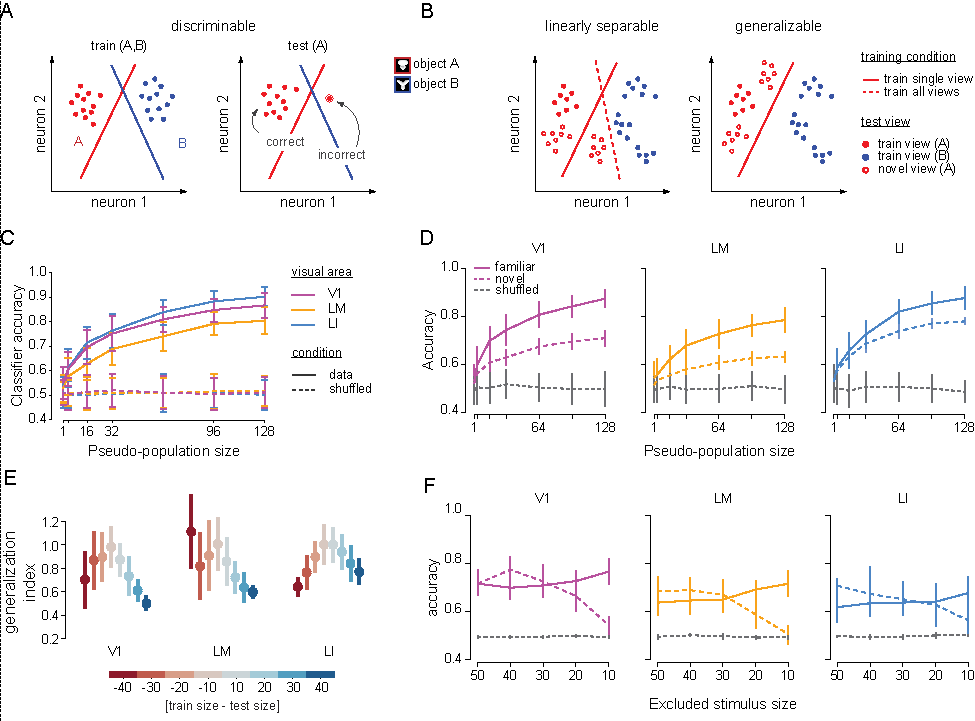
\includegraphics[width=0.9\textwidth]{figures/chapter_4/fig_4-4_neural_generalization/fig_4-4_neural_generalization.pdf}
    %\vspace{.1in}
    \centering
    \caption[Population representations of objects]{Linear separability and tolerance. 
    \textbf{A.} Schematic of discriminability for neural populations (adapted from \citet{Rust2010SelectivityIT}). A hypothetical population response for 1 presentation of an image as a point in N-dimensional space (example shows a population of size N=2 for illustration). Different trials of the same image (red) form a cloud in this N-D space, while trials of a different image (blue) form another cloud (left). The ability of the population to discriminate the images is proportional to how far apart the response clouds are. Linear classifier approaches identify the optimal hyperplane that separates one image (red) from the other (blue). Performance is measured as the proportion of times that response vectors fall on the correct side of the hyperplane (right). 
    \textbf{B.} \textit{Left}: A population that supports generalization under one test (dashed line) but fails under another (solid line) for different, novel views (red, open circles) of an object. \textit{Right}: A population that passes tests of generalization when testing on a single training condition (solid line in \textit{left}), as illustrated by the response vectors for both novel and trained views falling on the correct side of the hyperplane.
    \textbf{C.} Linear separability as a function of population size (see \textbf{B}, left) for V1, LM, and LI. Classifiers were trained on with responses from all sizes. Dotted, shuffled labels. Error bars, bootstrapped estimates of the 95\% CI of the mean accuracy. 
    \textbf{D.} Generalization test accuracy (see \textbf{B}, right) by population size for V1 (left), LM (middle), and LI (right). Classifiers were trained at 1 stimulus size, then tested on new samples of the same (black) or novel stimulus sizes (blue). Dotted lines and error bars as in \textbf{C}.
    \textbf{D.} Generalization score (ratio of novel to trained) split by the difference between train and test stimulus sizes (N=128 cells).
    \textbf{E.} Generalization test accuracy at each trained stimulus size. Classifiers were trained with 4 out of 5 stimulus sizes, then tested on different trials of the training size (black) or on new trials of the held-out, novel size (blue), for all combinations of train/test sizes. Error bars, SD across imaging sites. Dotted lines, shuffled labels.
    \label{fig:neural_generalization}}
\end{figure}


However, during behavior, the animal has access to much more than the activity of a single neuron. To determine the extent to which neural populations in rat visual cortex are inherently capable of representations that support discrimination and generalization, I took a population-based approach to compare areas V1, LM, and LI in awake, but untrained rats. Specifically, I trained linear SVMs with neural responses to these same object images to classify the responses as belonging to object A or object B \cite{Hung2005, Li2009, Rust2010SelectivityIT}. I then tested the classifiers on each of the two types of generalization tasks performed by the trained rats. 

Before testing the ability of each population to generalize across identity-preserving transformations, I first tested how well the objects could be discriminated from each other at each of the tested transformations. That is, if a given population failed to discriminate the objects at a given size, failure to generalize to that size would be trivial. For each imaging site, or set of simultaneously recorded cells, in each visual area, I trained linear classifiers to discriminate the two objects at each size, then scored accuracy on trials of the same condition that the classifier had never seen. To avoid trivial generalization due to poor baseline performance, only those populations with average test accuracies greater than accuracies calculated from shuffled object labels were included. 

To test discriminability of the two anchor objects, I first tested neural representations under a ``Train 1, test same'' regime: At each stimulus size tested, I trained classifiers to discriminate object A from object B. Overall, discrimination accuracy improved with increasingly larger stimulus sizes. This is consistent with previous single-unit studies of aggregated populations, though here we report performance for simultaneously recorded populations. This stimulus size dependence was present in all visual areas, and notably, overall performance was comparable across areas, as well. Specifically, average test scores were similar for populations in V1, LM, and LI, with mean scores in V1 and LM being slightly higher, but not significantly different, than LI (mean accuracy +/- std: V1, 0.73 +/- 0.08, n=9 sites; LM: 0.68 +/- 0.04, n=5 sites; LI: -0.64 +/- 0.09, n=4 sites; Mann-Whitney U test, p>0.05 corrected for multiple comparisons). As expected, I also found better discrimination accuracy for larger neural population sizes. Only imaging sites that passed this baseline discrimination task were included in further tests of generalization performance (see Methods). 

% Linear separability.
To quantify linear separability, I trained linear classifiers (support vector machines) to discriminate the two original objects from the neural responses in each area across different training regimes. The linear-readout scheme is important in that it is a simple, biologically plausible processing step that amounts to a thresholded sum taken over weighted synapses. This classifier approach does not provide a measure for the total information present in the population, but rather estimates the lower bound on the information explicitly accessible to the population to support the visual task. 

I started with a ``Train all, test all'' scheme:  Classifiers were first trained to discriminate object A from object B across all stimulus conditions, then tested on new samples of object A and object B. This is a measure of how separable object representations are across the different stimulus sizes. I found that classifier accuracy was comparable across areas V1, LM, and LI for all population sizes (Figure\ref{fig:neural_generalization}B). This held true even when restricting analyses to cells that had receptive fields overlapping with the stimulus from 0 to 100\%. % OVERLAP RFS?

% Arousal
% Increased shape selectivity could result in better linear separability, but decreased size tolerance could result in worse linear separability. REFREF.
% Arousal
% Consistent with the above results, we also found that linear separability of object representations was improved in high arousal states for V1, but was unaffected in LI, despite all areas exhibiting shifts in tolerance and selectivity in the same directions. However, LM also exhibited improved linear separability in high arousal states, like V1, despite there being no significant change in the linear relationship between selectivity and tolerance. This suggests that the tolerance/selectivity tradeoff may differentially affect object encoding and readout across visual areas.

Behaving animals achieved high levels of accuracy on completely novel, never-before-seen views of objects (see Figure\ref{fig:behavior_generalization}). To determine whether this might be true even in naive, untrained animals, I conducted a second test of generalization. Generalization to completely novel stimulus conditions was called the ``Train 1, test each of the others'' scheme:  I trained classifiers to discriminate object A from B at one stimulus size, then tested how well they generalized to each of the other, novel stimulus sizes. For example, if training at stimulus size \ang{10}, the test cases were 1 ``trained'' condition (different samples of stimulus size \ang{10}), and 4 ``novel'' conditions (the 4 other stimulus sizes that the classifier never saw). I observed accuracies well above chance for all visual areas, with overall accuracies improving for larger population sizes (Figure\ref{fig:neural_generalization}C). 

Notably, the difference in accuracy for trained versus novel conditions was qualiatatively smaller for LI, compared to V1 and LM (compared solid versus dashed colored line in Figure\ref{fig:neural_generalization}D). Given the earlier observation that single cells in LI exhibited a slightly higher size tolerance (Figure\ref{fig:selectivity_tolerance}), I asked whether generalization performance was dependent on which particular stimulus sizes the classifiers had access to during training. For each visual area, I calculated a generalization score, defined as the ratio of accuracy on trained conditions versus novel conditions. Since a high generalization score is trivially possibly for poor performance on both trained and novel conditions, I calculated this metric only for the largest, that is, best-performing population sizes for each visual area (n=128 cells). Logically, generalization might be better if the difference in training and testing conditions is small --- that is, training to discriminate object A from B at stimulus size \ang{10} might result in better generalization to stimulus size \ang{20}, compared to generalization to stimulus size \ang{50}. As expected, I found that generalization was best for training-testing regimes in which the difference in stimulus size at train and test was small (Figure\ref{fig:neural_generalization}E). Interestingly, I observed a slight asymmetry for V1 and LM populations: generalization was slightly worse if the novel stimulus size at test was smaller than the trained stimulus size. Generalization was symmetric about the difference between trained and novel conditions for LI.

To determine the extent to which generalization might be facilitated by the composition of stimulus conditions on which the classifier trains, I trained and tested linear classifiers for each visual area using all combinations of stimulus sizes. Specifically, I used a ``Train a subset, test 1 other'' scheme:  Each classifier was trained to discriminate object A from B using a range of stimulus sizes, namely all but 1 of the stimulus sizes, then tested on its ability to generalize to the remaining stimulus size. I found that while LI was robust to different training-testing combinations, V1 and LM were specifically sensitive to novel sizes if it was smaller than the trained stimulus sizes (Figure\ref{fig:neural_generalization}F, Wilcoxon signed-rank test, p<0.01). 


% Discussion. 
\section{Concluding remarks}
I characterized neural responses to complex visual objects that are known to elicit perceptual behaviors in trained rats. Specifically, I tested identity-preserving transformations (stimulus size) and identity-changing transformations (morphs) of two, complex object stimuli in naive, awake rats. Across all visual areas, I found broad similarities in many of the metrics tested. Single neurons in areas V1, LM and LI, showed wide ranges of morph selectivity and size tolerance (Figure\ref{fig:selectivity_tolerance}). Although size tolerance slightly increased from V1 to LM to LI, while morph selectivity decreased, the distributions of selectivity and tolerance metrics were similar. All areas also showed a trade-off between selectivity and tolerance, though this was more pronounced in areas LM and LI. As another measure of selectivity, I also characterized the extent to which single neurons could discriminate the two anchor objects (Figure\ref{fig:neurometric}). Although fewer cells in LI populations were selective for the object stimuli, compared to V1 or LM, all selective cells exhibited similar levels of discriminability across the three visual areas. 

Taking advantage of the access to facial features in head-fixed rats, I also characterized how neural tuning to the object stimuli were modulated by arousal states, as measured by changes in pupil size (Figure\ref{fig:arousal}). Intriguingly, I observed that although tolerance and selectivity metrics were similarly modulated across areas (higher arousal, higher shape selectivty and lower size tolerance), arousal affected the trade-off between the two only in V1; the negative correlation was unchanged for LM and LI populations. This raises the intriguing possibility that selectivity and tolerance may be decoupled in LM and LI, relative to V1, in that the trade-off between the two features is robust to arousal differences at the level of individual cells. In a similar vein, population decoding, as measured by linear separability, was improved in V1 for high compared to low arousal states, but unaffected in LM and LI. Nonetheless, the observed effects were small. Future studies incorporating additional facial features (whisking behavior, snout and mouth movements) may help identify a more complete representation of the many non-stimulus-related features that modulate neural activity.

Finally, to test the idea of increased linear separability of neural representations from lower to higher level visual areas, I performed a series of population readout analyses for areas V1, LM, and LI (Figure\ref{fig:neural_generalization}). Overall, I found that, similar to single neuron metrics, population readout was also similar across visual areas. Discriminability of the object stimuli was comparable across areas, reaching $\sim$80-90\% accuracy at the largest population sizes (n=128). Interestingly, I observed an asymmetry in generalization performance:  training classifiers to discriminate the objects from responses to presentations of larger stimulus sizes resulted in poorer generalization than when training on the smaller stimulus sizes. Importantly, this was not due to overall poor performance for smaller stimulus sizes, but was specific to test of generalization at novel, untrained sizes. Further exploration of these ideas are possible by closer examination of the separating hyperplanes in each of the training conditions, which may clarify which neurons are most informative when training on smaller stimulus sizes and why generalization is better under these regimes. 

In the context of visual object recognition, previous studies cite different visual areas as the most ``IT''-like, for example LI\cite{Tafazoli2017, Matteucci2019b} or TO\cite{Vermaercke2015, Vermaercke2014} or even LM\cite{Froudarakis2020}. Given the relatively inconsistent coverage of viral GCaMP expression across the many injection sites needed to cover the 5$mm$ window, area LL or area TO were only rarely located with confidence, and was thus excluded from these experiments. The ambiguities inherent in localizing small visual areas, given non-uniform viral expression, are largely overcome with the recent development of transgenic rats that express GCaMP in all neurons\cite{Scott2018}. I observed retinotopic reversals that were suggestive of visual areas beyond the three areas that are the focus of this study, and future experiments may be better able to apply many existing tools to more thoroughly characterize the extent and range of extrastriate visual areas in the rat. 

Nonetheless, the three areas under study did not exhibit clearly separable functional differences, as observed even in the earlier stages of the primate ventral stream. Although I observed several key signatures thought to be important for computations underlying visual object recognition, \textit{e.g.}, shape selectivity, transformation tolerance, and linear separability, the three visual areas were comparable in most regards. Future studies that take advantage of large-scale population recordings in awake rats should include a much larger range of object stimuli than the present study could provide. Since the goal of the experiments described here and in previous chapters was to provide foundational characterizations using optical methods, only a limited set of object stimuli could be tested. It is thus possible that the visual areas under study may exhibit more divergent feature selectivity when a richer stimulus set is used. 

In conclusion, the results of the present study suggest that rat visual cortex exhibits diverse response properties to visual object stimuli, some of which appear to be relevant for understanding how tolerant visual object representations are formed in a non-primate brain like the rodent. The absence of a clear functional separation of the three visual areas into a distinct and hierarchically-organized system, as observed in the primate ventral path, raises many more questions about the ways in which the rodent visual system has specializations distinct from the primate system. As shown by the growing number of discoveries in mouse visual cortex, it will be exciting to explore the neural computations and behaviors that are more ethologically relevant for a rat navigating a complex visual environment. 
